\documentclass[11pt]{article}

\usepackage[left=2cm, right=5cm, top=2cm]{geometry}
\usepackage[T1]{fontenc}
\usepackage[polish]{babel}
\usepackage[utf8]{inputenc}
\usepackage{lmodern}
\usepackage{amsfonts}
\usepackage{ragged2e}
\usepackage{graphicx}
\usepackage{calc}
\usepackage{amsmath}
\usepackage{csquotes}
\newlength{\depthofsumsign}
\setlength{\depthofsumsign}{\depthof{$\sum$}}
\newlength{\totalheightofsumsign}
\newlength{\heightanddepthofargument}

\newcommand{\nsum}[1][1.4]{
    \mathop{
        \raisebox
            {-#1\depthofsumsign+1\depthofsumsign}
            {\scalebox
                {#1}
                {$\displaystyle\sum$}
            }
    }
}

\selectlanguage{polish}

\title{Zadanie 4.}
\date{29 września 2018}
\author{Paweł Balawender}

\begin{document}
\maketitle

\section*{Problem}
\begin{justify}
Szachownicę o wymiarach $2018 \times 2018$ przykryto przy pomocy jednej
kwadratowej płytki o wymiarach $2 \times 2$ oraz $\frac{2018^2-4}{5}$
prostokątnych płytek o wymiarach $1 \times 5$ w taki sposób, że każde pole szachownicy jest przykryte
przez dokładnie jedną płytkę (płytki można obracać). Wykazać, że płytka $2\times2$ nie przykrywa żadnego pola o krawędzi zawartej w brzegu szachownicy
\section*{Dowód}
Dla uproszczenia nazwijmy płytki o wymiarach $1 \times 5$ klockami.
Płytka o wymiarach $2 \times 2$ powoduje, że $klocki$ nie będą mogły być ustawione jeden obok drugiego
(tj. tak, że mają z innym klockiem 5 wspólnych krawędzi pól, które przykrywają), wprowadzi natomiast pewną nierówność: w wierszach szachownicy,w których leży płytka $2 \times 2$, przynajmniej 1 ($2016 \mod 5 \equiv 1$) klocek będzie musiał być ustawiony pionowo tj. w tylko jednej kolumnie szachownicy.
W pozostałych wierszach będą to przynajmniej 3 ($2018\mod 5 \equiv 3$) klocki (analogiczna sytuacja zachodzi dla kolumn - będą musiały być one dopełniane klockami ułożonymi poziomo). Prowadzi to do powstania pewnego dysonansu, który uniemożliwi wyparkietowanie tej figury.
Jeśli klocek zostanie ułożony tak, że odległość jednego z jego końców od krawędzi szachownicy nie jest podzielna przez 5, to będą potrzebne klocki zorientowane w tym kierunku, w którym ich szerokość wynosi 1, tak, by pokryć tę \textit{resztę z dzielenia}. To z kolei spowoduje, że te \textit{pomocnicze} klocki będą ułożone w nielosowych
kolumie lub wierszu zgodnymi z ich kierunkiem, prowadząc do tego, że ponownie będzie trzeba użyć \textit{pomocniczych} klocków etc. etc. --- łatwo spostrzec, że jest to problem rekursyjny. Skoro rozmiary klocków, ilość wierszy i kolumn są stałe, to nie powstanie w tej figurze kolejna nierówność, która
złożona z tę wprowadzoną przez płytkę $2 \times 2$ doprowadzi do sytuacji,  w której będzie można \enquote{bez reszty} wyparkietować resztę kolumny/wiersza zgodnego z kierunkiem tego nierówno włożonego klocka. Wyjściem z tej sytuacji jest \enquote{owinięcie} płytki $2 \times 2$ czterema blokami po trzy klocki, w taki sposób, że z czterech stron płytki $2 \times 2$ będą po trzy 
klocki sąsiadujące ze sobą dłuższym blokiem (powstanie swego rodzaju swastyka wykonana z klocków, z płytką $2 \times 2$ w centrum). W wyniku wykonania tej operacji otrzymamy
nową figurę o wymiarach $(3+2+3 \;\times\;  3+2+3)$, tj. $8 \times 8$. Wtedy jeśli konstrukcja taka będzie ustawiona wewnątrz kwadratu w taki sposób, że będzie ona dzielić kolumny i wiersze,
w których leży, na części o długości podzielnej prez 5, to całą tę figurę opisaną w zadaniu będzie można wyparkietować: będzie można ją podzielić na prostokąty, których boki są podzielne przez 5, więc zawsze będzie można je wyparkietować, chociażby poprzez konsekwentne ustawianie klocków obok siebie lub jeden za drugim.

Podsumowując, by wyparkietować tę figurę, płytka $2 \times 2$ musi być otoczona konstrukcją wykonaną z klocków - nigdy nie będzie więc ona miała wspólnej krawędzi z krawędzią szachownicy.

Oglądowy rysunek konstrukcji umożliwiającej wyparkietowanie figury z zadania: \linebreak
\center{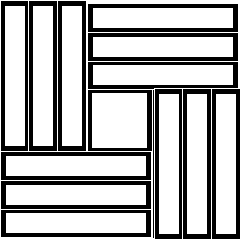
\includegraphics{OM4.png}}
\end{justify}
\end{document}